\documentclass[border=10pt]{standalone}

\usepackage{tikz}
\usepackage{xcolor}
\usepackage{mathtools}

\usetikzlibrary{shadings,shadows,shapes.arrows}

\begin{document}
\begin{tikzpicture}[scale=1, transform shape]
    \draw [draw=black!20, line width=2pt, path picture={\node (source) at (path picture bounding box.center)
        {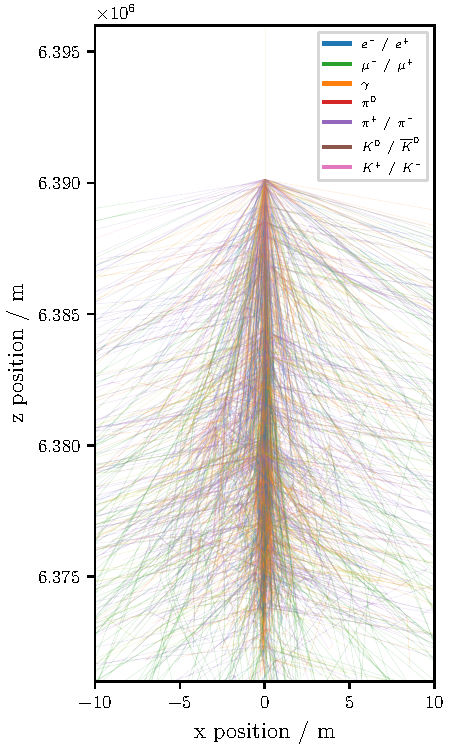
\includegraphics[height=4.7cm]{./shower_proton.pdf}};} ] (0,0) rectangle (3,5);
    \node (proton) at (1.5, 5.3) {\small $p$ induced};

    \draw [draw=black!20, line width=2pt, path picture={\node (source) at (path picture bounding box.center)
        {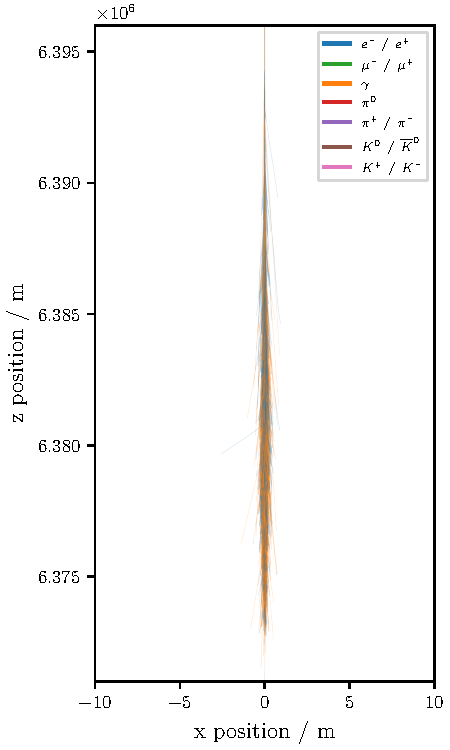
\includegraphics[height=4.7cm]{./shower_electron.pdf}};} ] (3.3,0) rectangle (6.3,5);
    \node (proton) at (4.8, 5.3) {\small $e^-$ induced};
\end{tikzpicture}
\end{document}
